\documentclass[letterpaper]{article}
% Required Packages
\usepackage{aaai}
\usepackage{times}
\usepackage{helvet}
\usepackage{courier}
\usepackage{changepage}
\usepackage{graphicx}
\usepackage{amsmath}
\graphicspath{ {imgs/} }
\setlength{\pdfpagewidth}{8.5in}
\setlength{\pdfpageheight}{11in}
%%%%%%%%%%
% PDFINFO for PDFLATEX
% Uncomment and complete the following for metadata (your paper must compile with PDFLATEX)
\pdfinfo{
/Title (Identifying Features for Bluff Detection in No-Limit Texas Hold'em)
/Author (Razvan Ranca)
/Keywords (poker, heads-up, no-limit, texas hold'em, opponent modelling, bluff)
}
%%%%%%%%%%
% Section Numbers
% Uncomment if you want to use section numbers
% and change the 0 to a 1 or 2
\setcounter{secnumdepth}{0}
%%%%%%%%%%
% Title, Author, and Address Information
\title{Identifying Features for Bluff Detection in No-Limit Texas Hold'em}
\author{Razvan Ranca\\
School of Informatics, University of Edinburgh\\
10 Crichton Street, Edinburgh, Scotland, United Kingdom\\
\emph{ranca.razvan@gmail.com}
}
\nocopyright
%%%%%%%%%%
% Body of Paper Begins
\begin{document}
\maketitle

\begin{adjustwidth}{10pt}{10pt}
\section{
\fontsize{10pt}{12pt} 
\selectfont 
Abstract}
\fontsize{9pt}{10pt}
\selectfont
Poker is increasingly becoming an area of interest in AI research, partly because of the complex qualities it exhibits which are absent from more traditionally studied games, such as chess. One of the most difficult but also most important aspects of poker is the need to infer information about your opponent while also handling his attempts at disinformation. This problem of ``opponent modelling" is a central aspect of poker agent design and has been approached in many different ways. In this paper we focus on one subset of the opponent modelling problem, namely that of bluff detection. We explore the effectiveness of different feature sets towards this task and test the ease with which the bluffs of various poker agents can be detected.
\end{adjustwidth}

\section{
\fontsize{12pt}{15pt} 
\selectfont
Introduction}
\fontsize{10pt}{12pt} 
\selectfont
Poker is a partially observable, dynamic, stochastic, mutiagent game, and therefore a challenging and interesting domain for artificial intelligence research. The large number of possible dealt cards and the large number of possible player actions gives poker a search space with a very large branching factor, the exploration of which is infeasible for classic AI techniques. The new approaches that must be developed to handle these issues promise to prove useful in a large range of practical applications.

One possible technique for designing a poker agent is the game theoretic approach which calculates an approximation to the Nash equilibrium strategy \cite{P11,P12}. This method has previously proved successful, for instance in the Annual Computer Poker Competitions (ACPC)\footnote{ACPC website: http://www.computerpokercompetition.org/}. This approach, however, suffers from a serious flaw. By trying to play an equilibrium strategy, the agent is trying to \emph{minimize losses} which, in most poker scenarios, is the wrong thing to do. By trying to minimize losses, the agent allows his opponents to play to \emph{maximize gains}, without any fear of repercussions. Some consequences of this weakness have been observed in the ACPC results, where equilibrium bots have managed to lose the overall bankroll challenge despite defeating every single opponent. In order to address this issue, agents have to play exploitatively, meaning they have to capitalize on the weaknesses of their opponents. Any such exploitative approach will need a way to model the behavior of its opponents so that it may try to understand their actions.

If we are to define an opponent model, we must first make generalizing assumptions about the opponent's behavior. This necessity is caused by the huge search space of poker, which makes it unlikely that we will encounter the same exact situation twice. In order to make these assumptions, we must identify the most important aspects of the opponent's play, namely those aspects which can be best used to predict his future behavior.

In the rest of this paper we will identify several possible features and look at their distribution over bluffs and non-bluffs. We will then try to quantify both the information gained from using individual features and the predictive power of using combinations of them. Lastly we will look at the convergence rates on our predictions, and see whether the features could reasonably be used for bluff detection during real play. First, however, we will take a look at previous opponent modelling approaches.


\section{
\fontsize{12pt}{15pt} 
\selectfont
Opponent Modelling Review}
\fontsize{10pt}{12pt} 
\selectfont
Exploitative agents can generally be classified as either static or adaptive, both of which incorporate an opponent model, which usually has a large impact on the overall effectiveness. \cite{P1} 

The static agents rely on a pre-computed exploitative strategy that is stored and used when appropriate during play. The simplest form of this agent uses an opponent model called a ``frequentist best response" which works by analyzing a large history of games, and storing the statistical best response at every encountered situation. In order to be tractable, the poker search space is mapped to a lower dimensional equivalent using such methods as grouping the possible starting hands into several buckets, based on the probability of winning at showdown. \cite{P4,P9}. During play the bot will map the current situation to the same lower dimensional space and play the pre-computed best response stored there. When presented with a static opponent and a large database of this opponent's play history, the frequentist best response method will achieve close to maximal possible exploitation.This model, however, is quite brittle and if the opponent's strategy changes even slightly the performance can drop drastically  \cite{P3}. Robustness can be gained by mixing the above method with an e-Nash equilibrium bot. This can be done by assuming the opponent will play according to our model some percentage of the time, and that he will play some unknown strategy the rest of the time. The equilibrium strategy can be calculated for this new scenario, which will be a compromise between the pure exploitative and the pure equilibrium extremes  \cite{P2,P3}. A final refinement to the above solution was explored in  \cite{P5}, where the probability that the opponent will or will not respect our model is based on how confident we are of our model in the current position in the game tree. This is an improvement since we will have more confidence in our opponent model in some situations than others.

The adaptive agents, instead, do an incomplete information game tree search. This approach involves a key trade-off between exploitation and exploration. It is tempting to always pick the most exploitative option, but this may lead to encountering fewer unique situations and therefore having a weaker opponent model. Different solutions to this problem have been attempted in  \cite{P6} and  \cite{P7}. Another issue involved in designing adaptive models is that they must get decent results after dozens of hands rather than thousands. Because of this, if the frequentist best response method is to be used, the lower dimensionality space to which the world is mapped needs to be exceedingly simple, which limits the effectiveness of the agent. Relatively good results have been obtained by using a series of successively simpler world models and inter-linking them so they share information as to make optimal use of every observed hand.  \cite{P6,P8}. More traditional machine learning methods have also been applied to this problem, such as reinforcement learning \cite{P13} and neural networks \cite{P9}. For the latter, the author notes positive results when evaluated against human players despite the fact that the large computational cost meant he could only perform the game tree search on the current betting round.

Finally, there are mixed approaches such as  \cite{P10} which first pre-calculate several disjoint static exploitative strategies, each corresponding to a class of players, and during play attempt to classify their opponent into one of these classes.

These approaches all have the feature selection problem in common. In the static case, the designer must select the features on which to base his lower dimensional mapping, and in the adaptive case the agent must decide which features it will first expand in the incomplete game tree search.

\section{
\fontsize{12pt}{15pt} 
\selectfont
Data Preparation and Features Used}
\fontsize{10pt}{12pt} 
\selectfont
Our data consists of the logs of the 2012 ACPC no-limit hold'em competition (including both the instant run-off and the total bankroll results). Since these logs contain a large amount of hands, we take a conservative approach in identifying bluffs and non-bluffs. Specifically, we look for hands in which the flop contains 3 cards of the same suite and one of the players makes a raise upon seeing the flop. This is a classic bluff scenario, in which the player who raises may genuinely have the flush or may try to convince his adversary that he has the flush. We further filter these hands as to disregard situations in which the player who raises has only one matching card as, in that case, it's unclear how much of a bluff his raise is. This leaves us with two clear categories, a bluff when the player who raises has no card of the right suite, and a non-bluff when said player has already made the flush. After the filtering we are left with $\sim$376,000 hands played amongst the 11 players.

We next analyze 8 features which a human might use when making a decision regarding the opponent's hand strength. These features are:

\begin{description}
  \item[Position:] whether the adversary plays first in this hand.
  \item[Pot amount:] the amount of money currently on the table.
  \item[Raise/Pot:] how large the opponent's raise was in relation to the pot at the time of his bet.
  \item[Flop strength:] the strength of the flop cards. This is measured by making all possible 5 card hands containing the flop cards and averaging their strength\footnote{The strength of a hand is calculated using the \emph{poker-eval}\\ library (http://pokersource.sourceforge.net/)}.
  \item[Number of pre-flop raises:] how many times the opponent has raised pre-flop.
  \item[Average pre-flop raise/pot:] on average, how aggressive the opponent's pre-flop raises were. This is 0 if there were no pre-flop raises.
  \item[Number of hands played:] how many hands have been played in this match so far. Since the total number of hands in a match is fixed, this indicates at what stage in the match the agents are.
  \item[Proportion won in similar hands:] how successful the adversary has been in ``similar" hands during the match. Similar hands are defined as hands that fit the filtering criteria described above. Success is measured as the amount of money won by the adversary divided by the total amount of money played in these hands. 
\end{description}

The features' distributions over the bluff and non-bluff classes are shown next in Figures 1 to 8. Note that ``all" means the amalgamation of all filtered hands and is therefore a combination of the 11 bots. As such ``all" can be viewed as somewhat of a generic agent, incorporating several strategies.

\onecolumn
\begin{figure}[H]
    \centering
    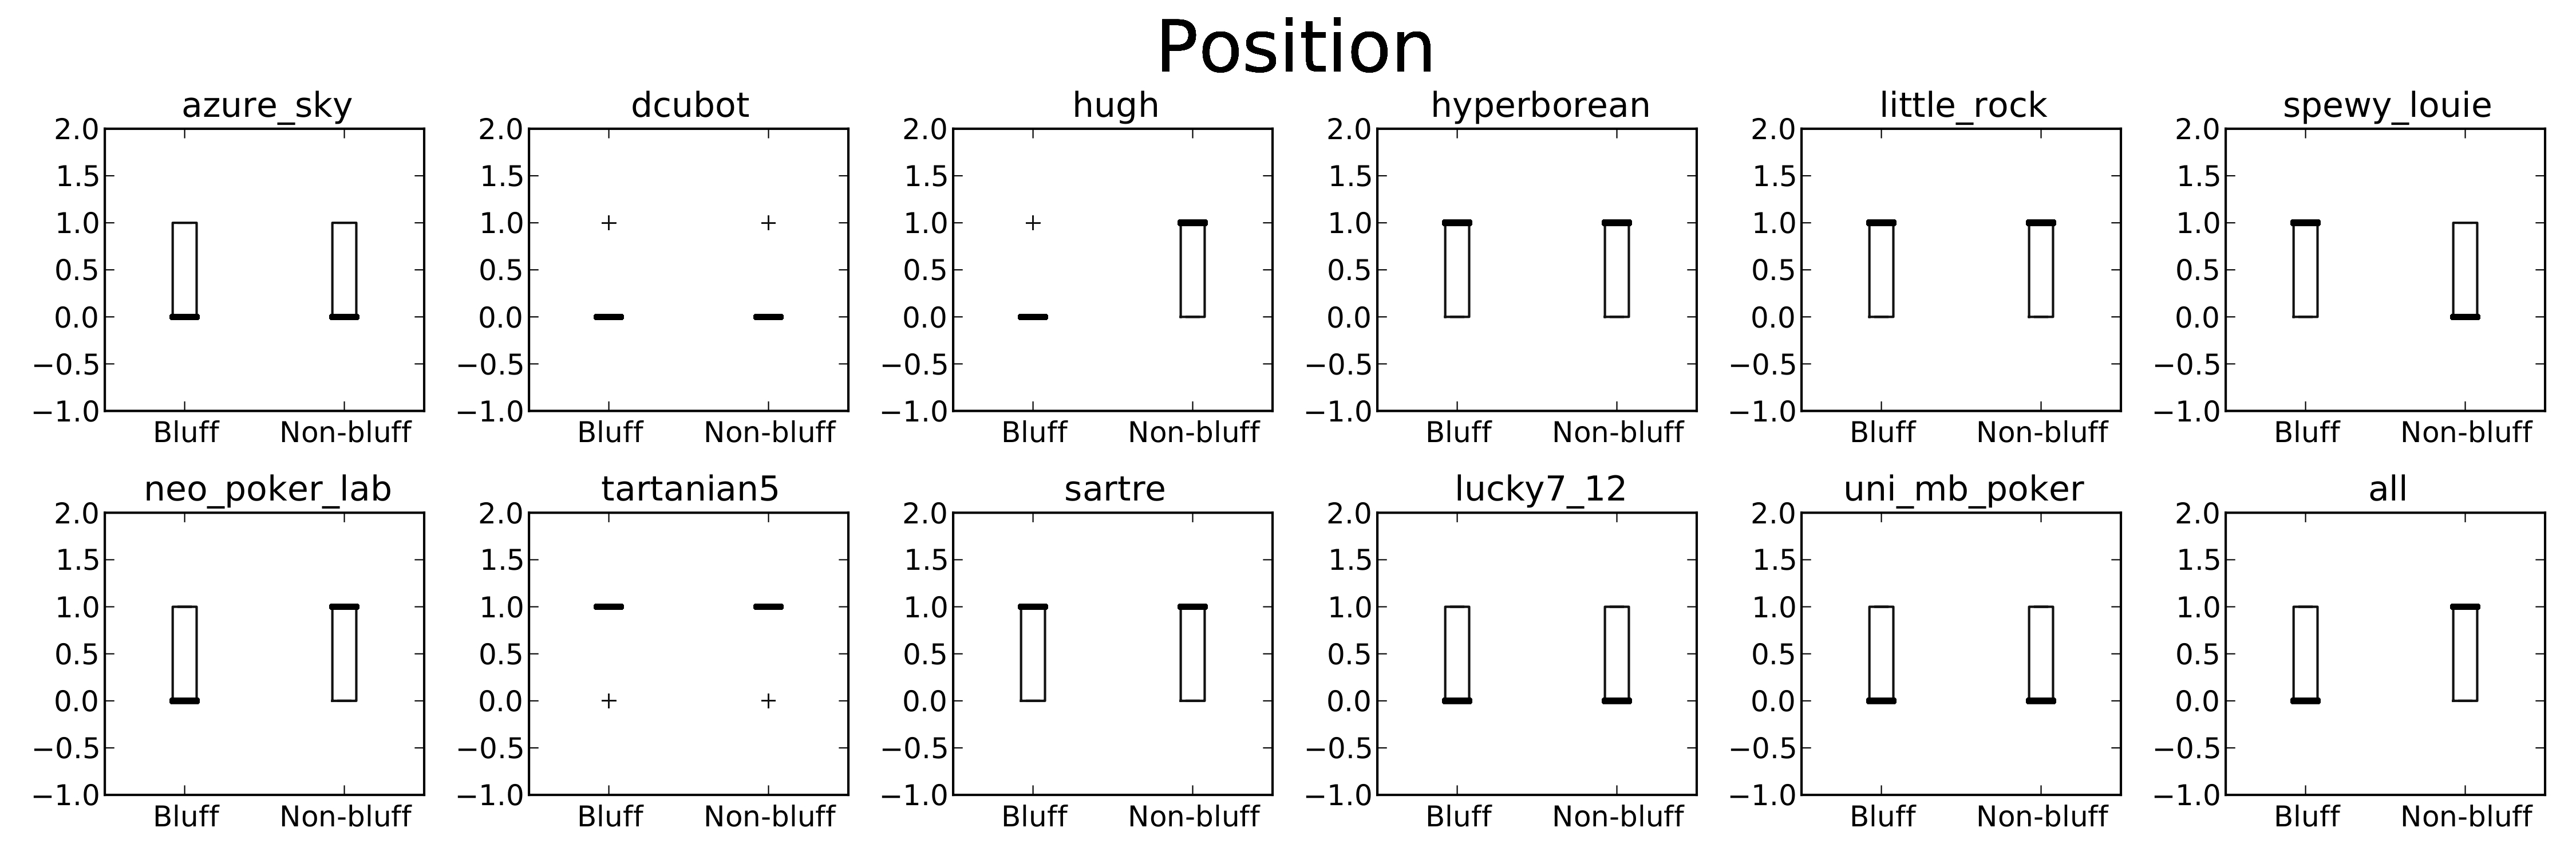
\includegraphics[width=\textwidth,natwidth=610,natheight=642]{posBW.jpg}
    \caption{Position is 0 if the adversary plays first and 1 otherwise. For hugh, spewy\_louie  and neo\_poker\_lab the means of the distributions vary between the two classes, which can be exploited. }
    \label{fig:pos}
\end{figure}
\begin{figure}[H]
    \centering
    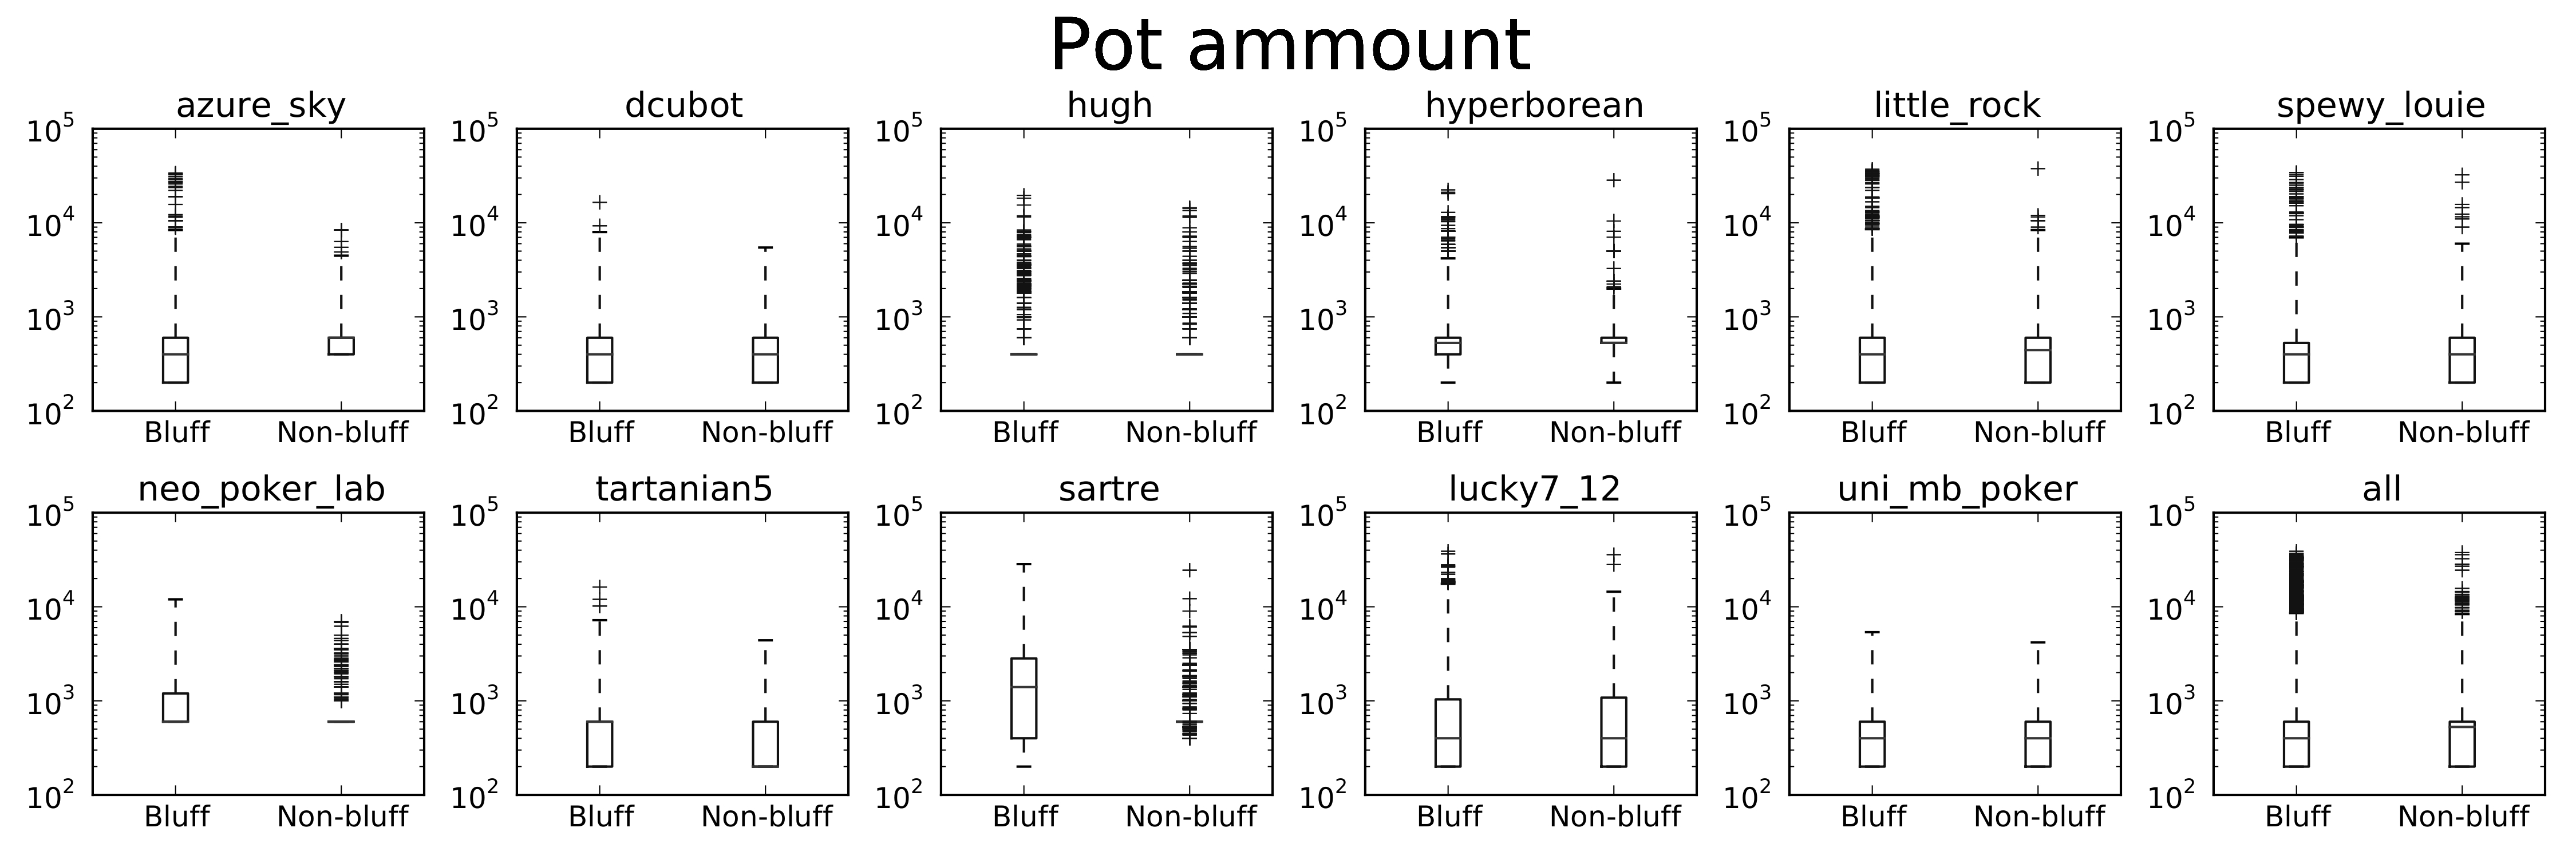
\includegraphics[width=\textwidth,natwidth=610,natheight=642]{potVarBW.jpg}
    \caption{We can see some discrepancies in the pot amounts. azure\_sky, for instance, seems to always be bluffing if the pot is under a certain amount. This is probably because if the bot actually had a suited hand pre-flop he would have bet more.}
\end{figure}
\begin{figure}[H]
    \centering
    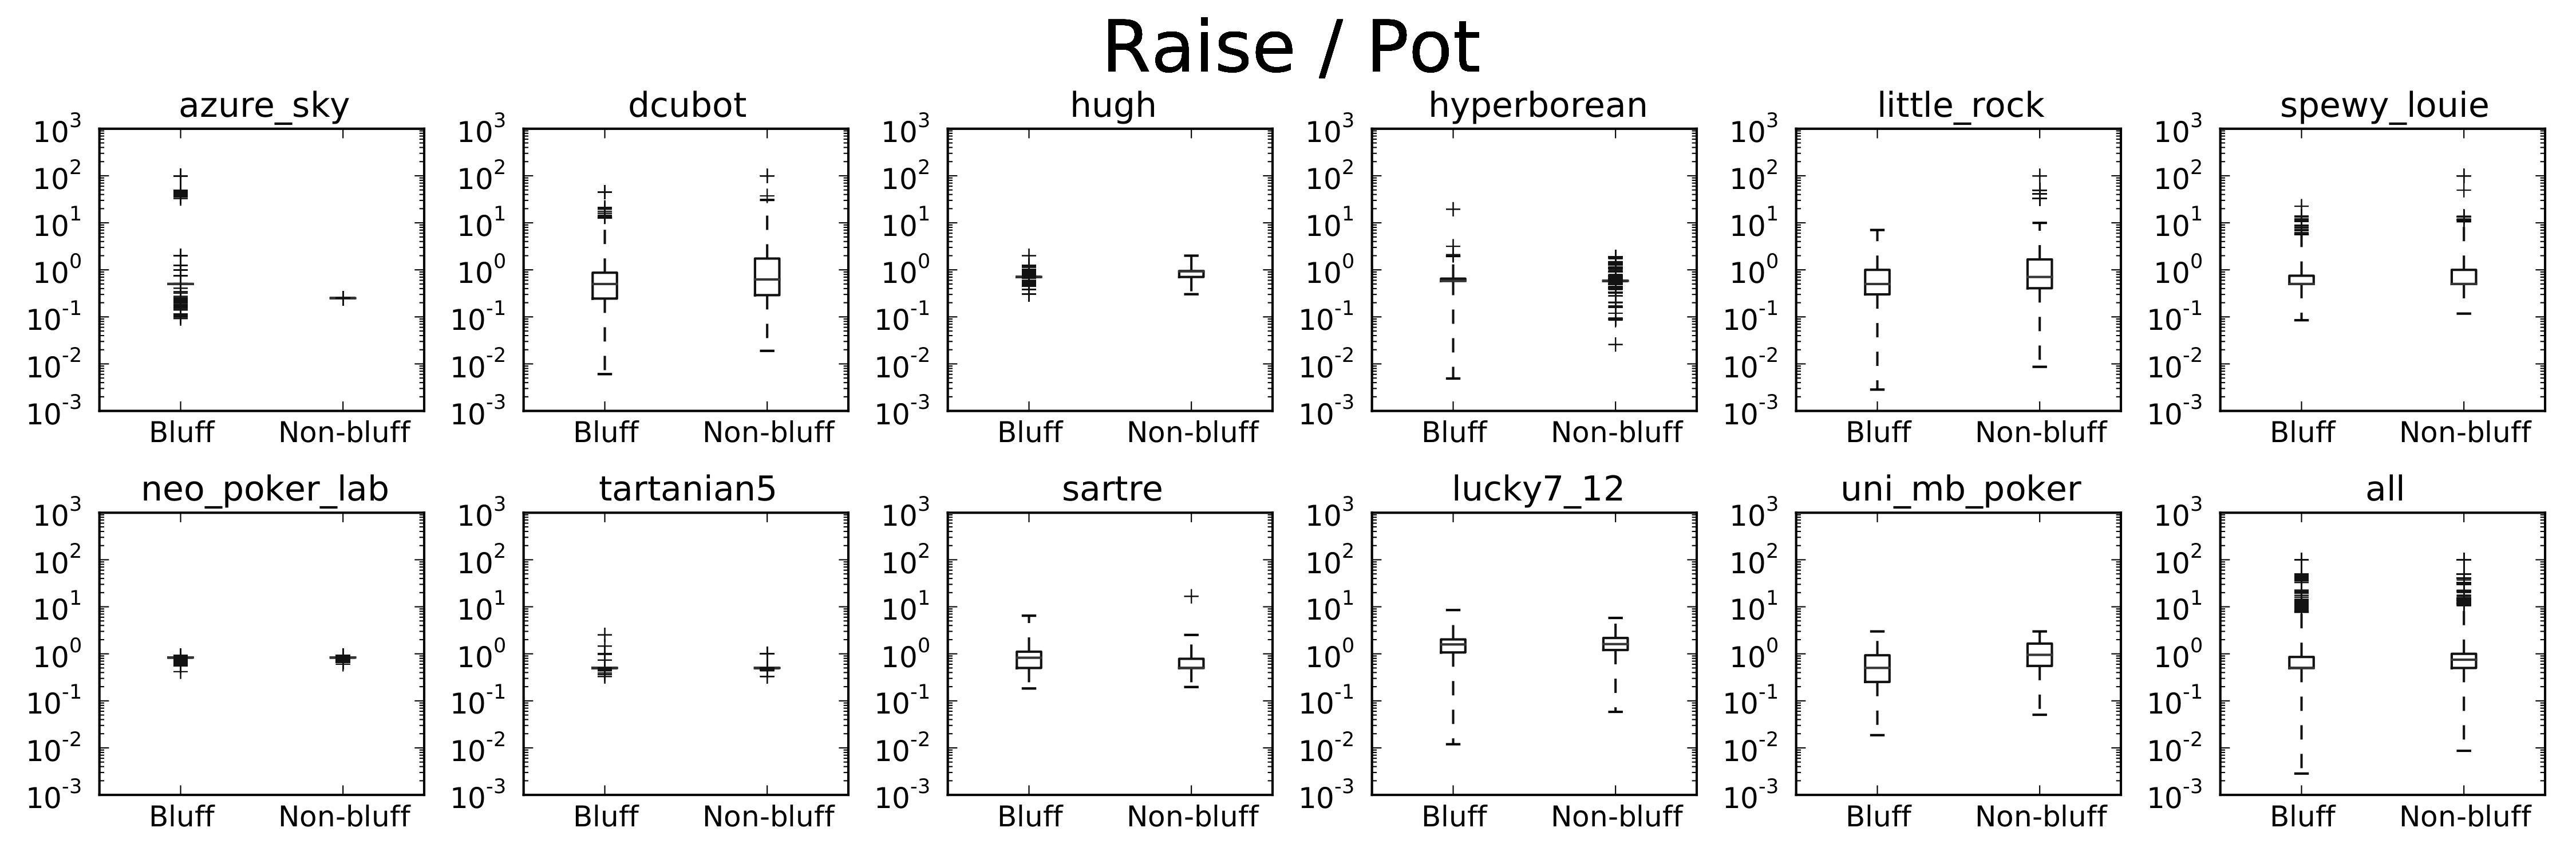
\includegraphics[width=\textwidth,natwidth=610,natheight=642]{raisePotVarBW.jpg}
    \caption{Several other discrepancies here. It seems that azure\_sky almost always bets the same proportion when not bluffing. Additionally, in general, the bots seem to bet more when not bluffing.}
\end{figure}
\clearpage
\begin{figure}[H]
    \centering
    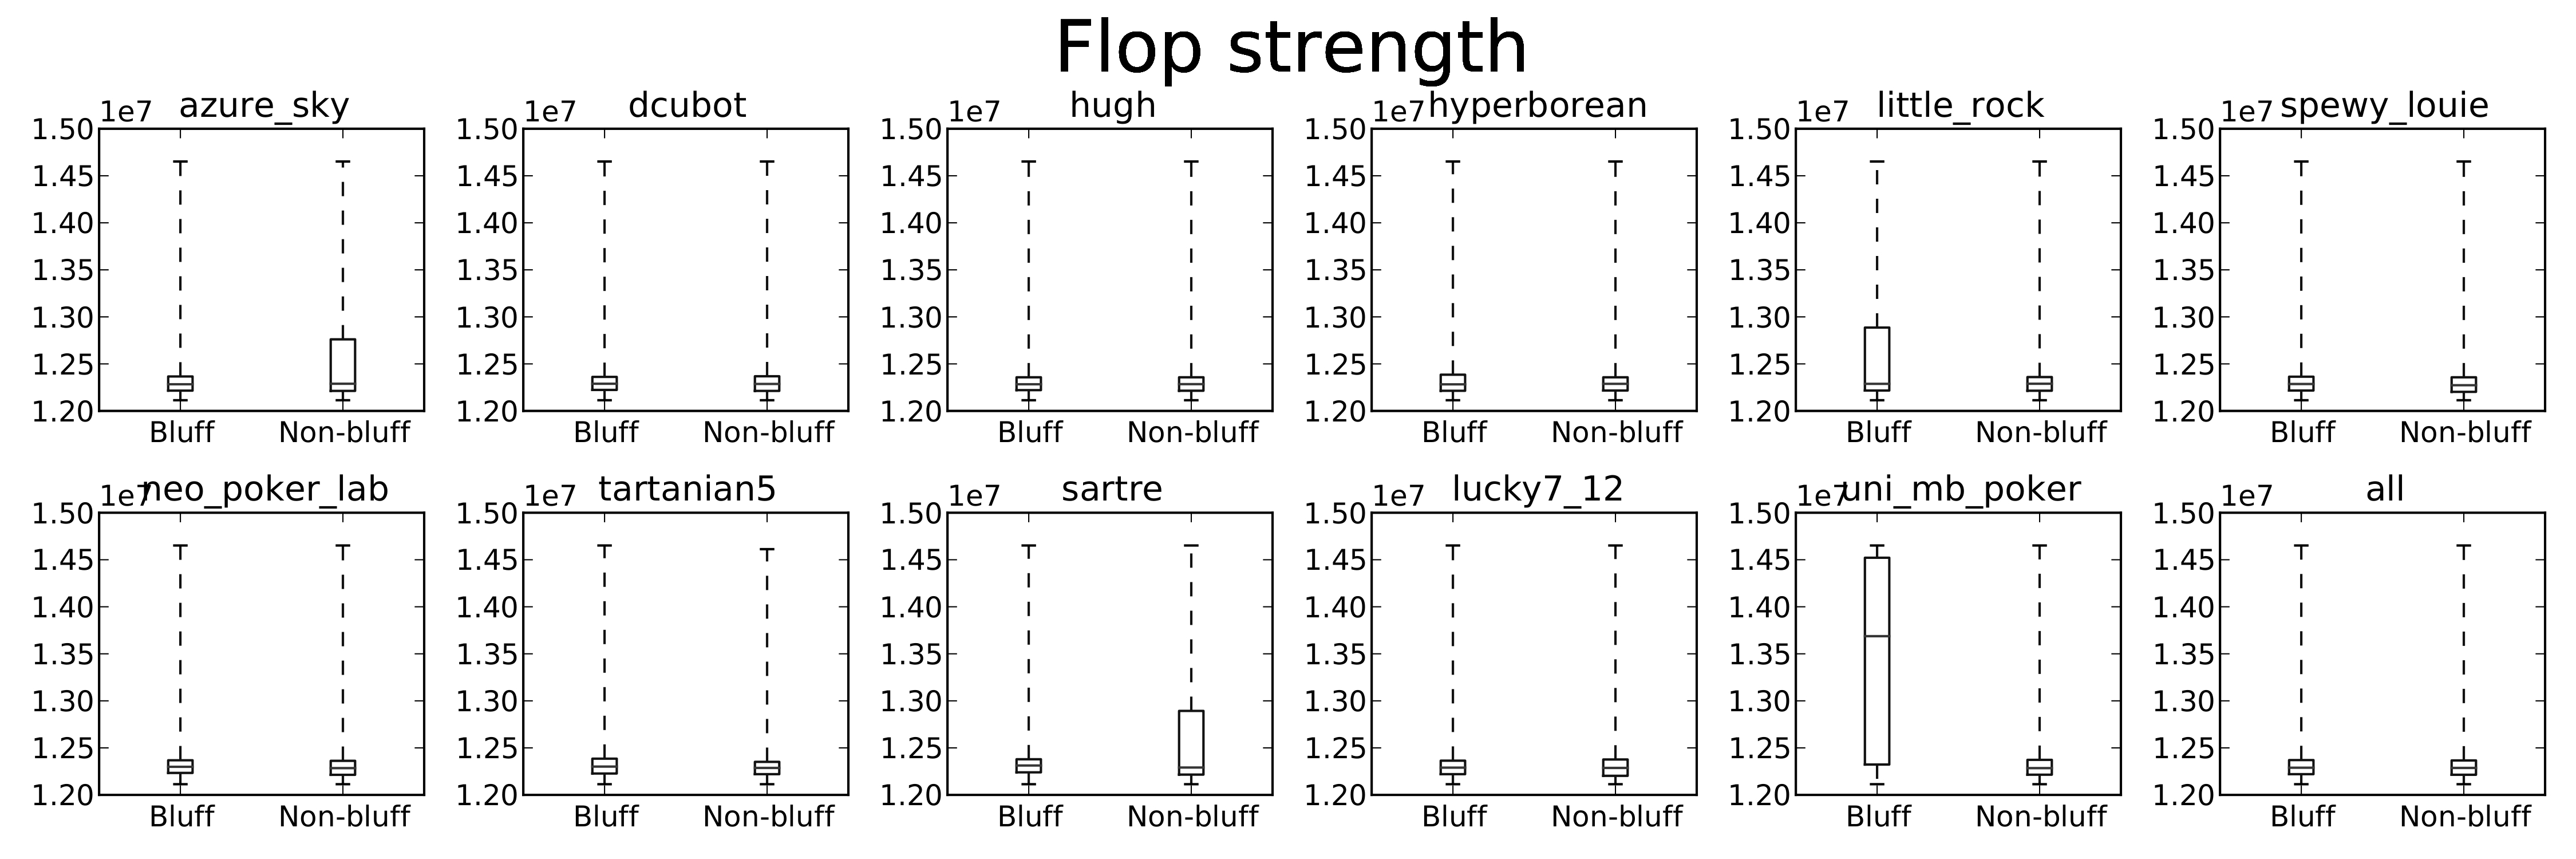
\includegraphics[width=\textwidth,natwidth=610,natheight=642]{flopStrengthBW.jpg}
    \caption{This measure appears to only work well on a couple of bots. We can see that, for instance, uni\_mb\_poker much prefers to bluff when the flop is stronger, probably because the bot considers it easier to scare his opponent in these scenarios.}
\end{figure}

\begin{figure}[H]
    \centering
    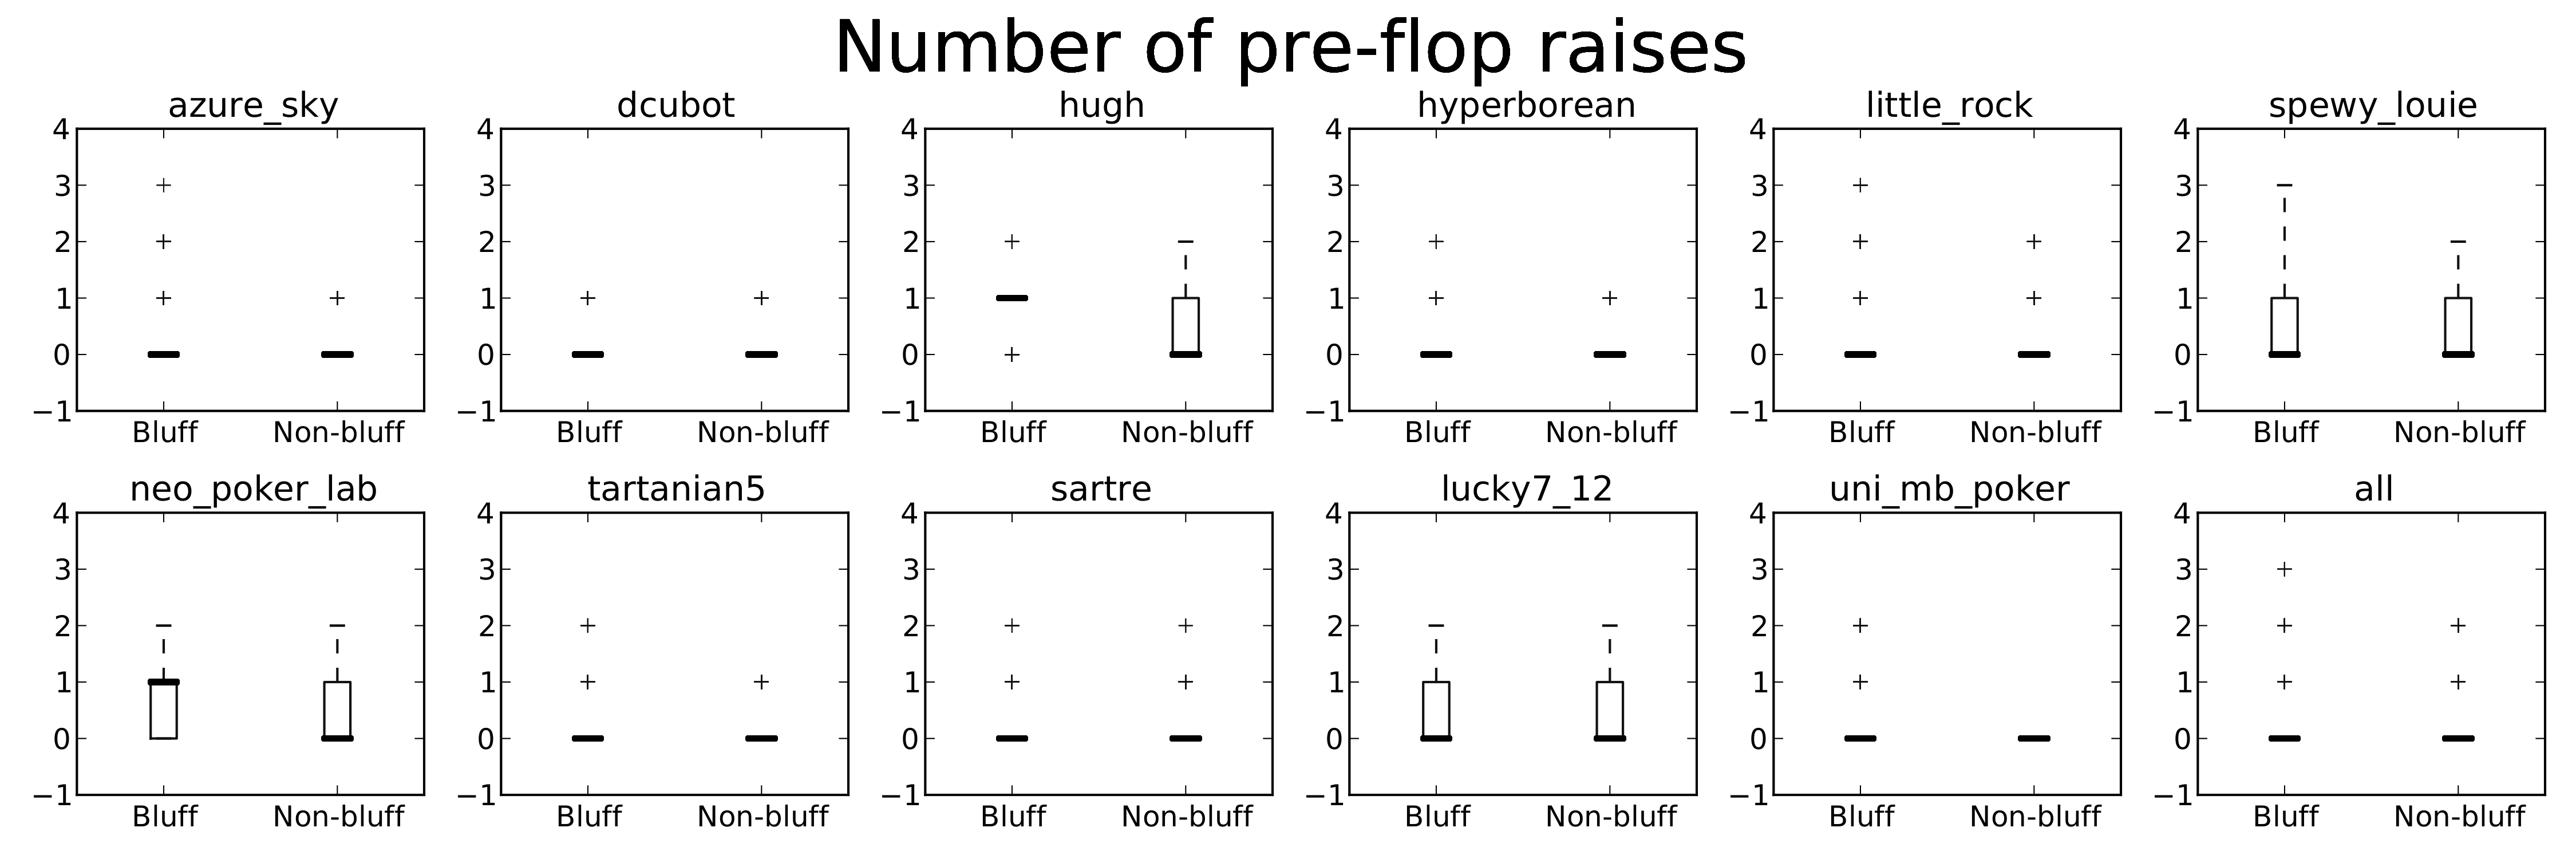
\includegraphics[width=\textwidth,natwidth=610,natheight=642]{noRaisesBW.jpg}
    \caption{We can notice here that several bots are more likely to be bluffing if they played aggressively pre-flop. This is likely because they believe their aggressive behavior can be exploited to scare the opponent.}
\end{figure}

\begin{figure}[H]
    \centering
    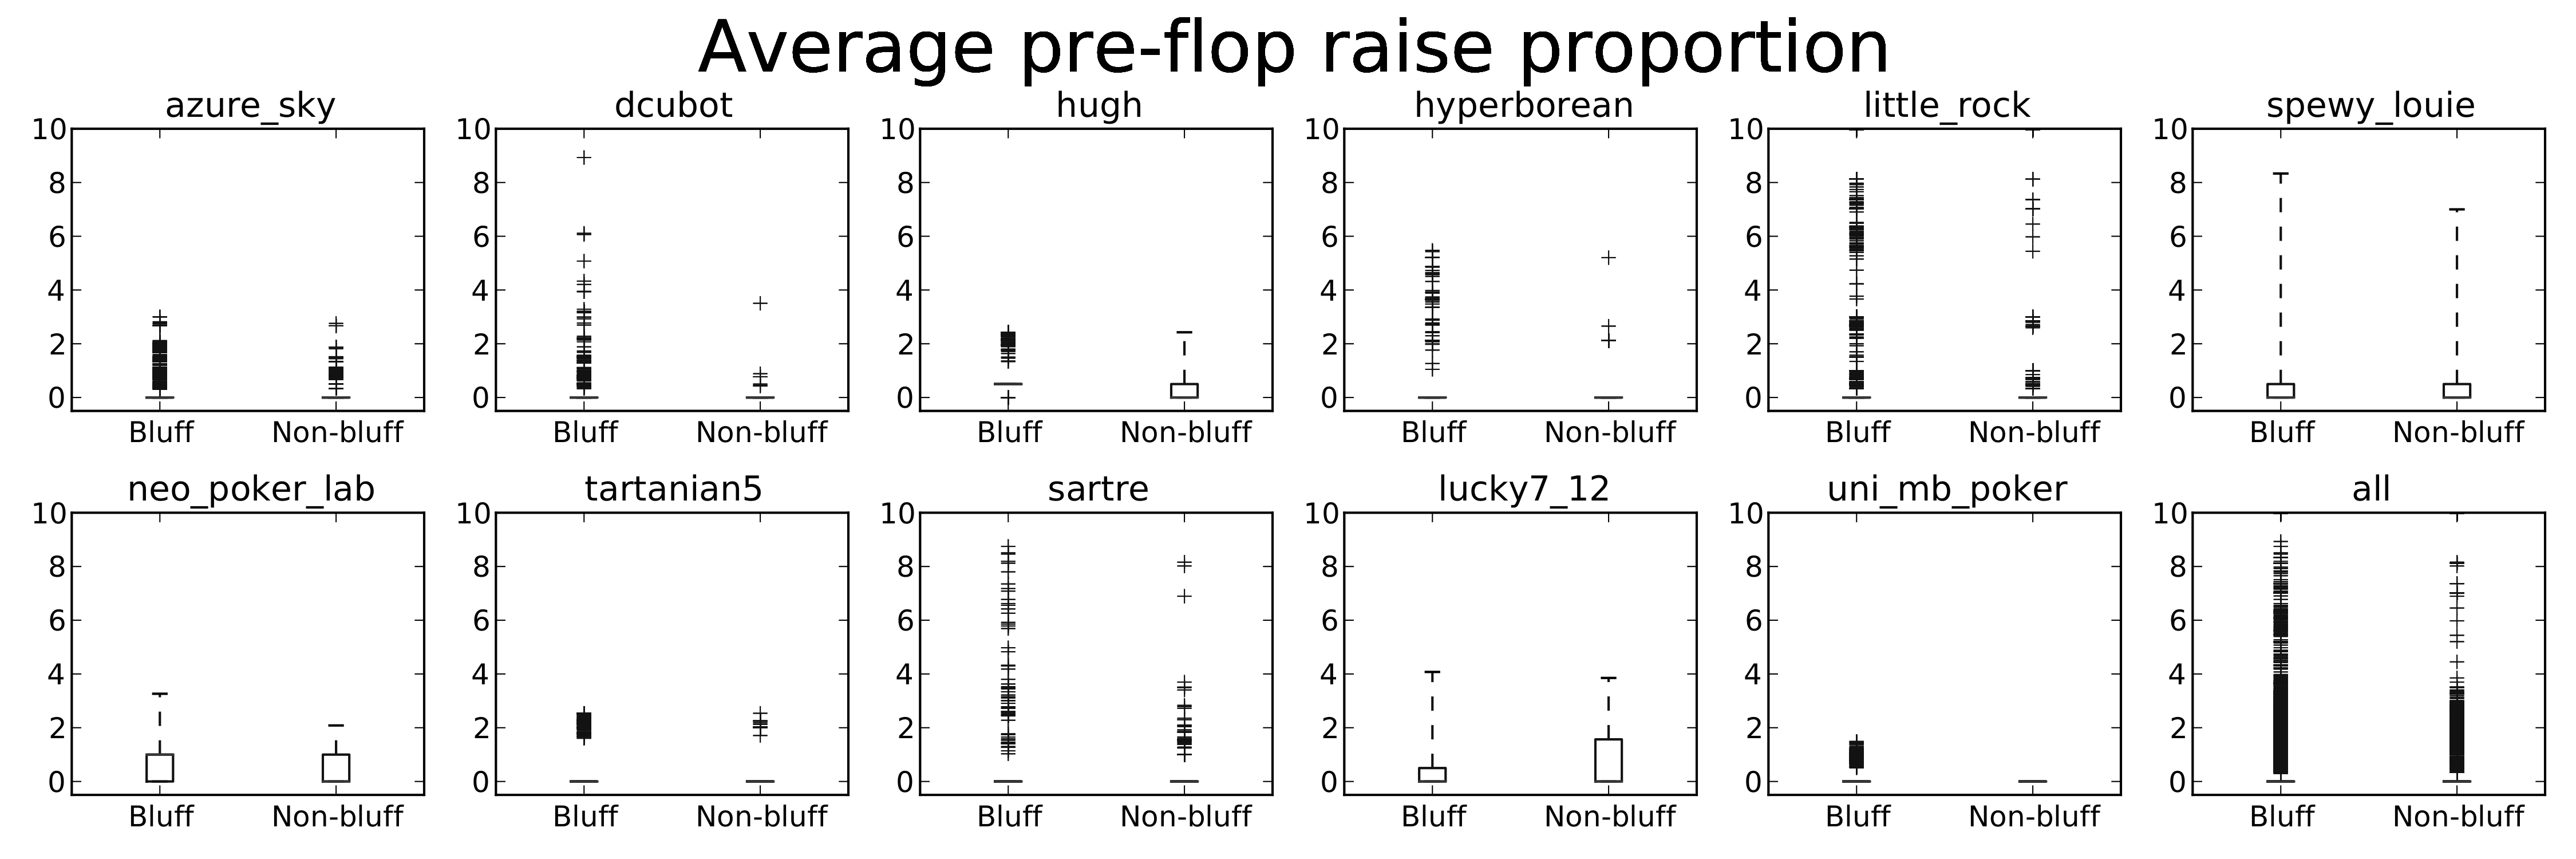
\includegraphics[width=\textwidth,natwidth=610,natheight=642]{avgPreRaiseBW.jpg}
    \caption{The trend observed in Figure 5 is repeated here. The only bot to reverse the trend is lucky7\_12 who seems to take a more conservative approach.}
\end{figure}

\clearpage

\begin{figure}[H]
    \centering
    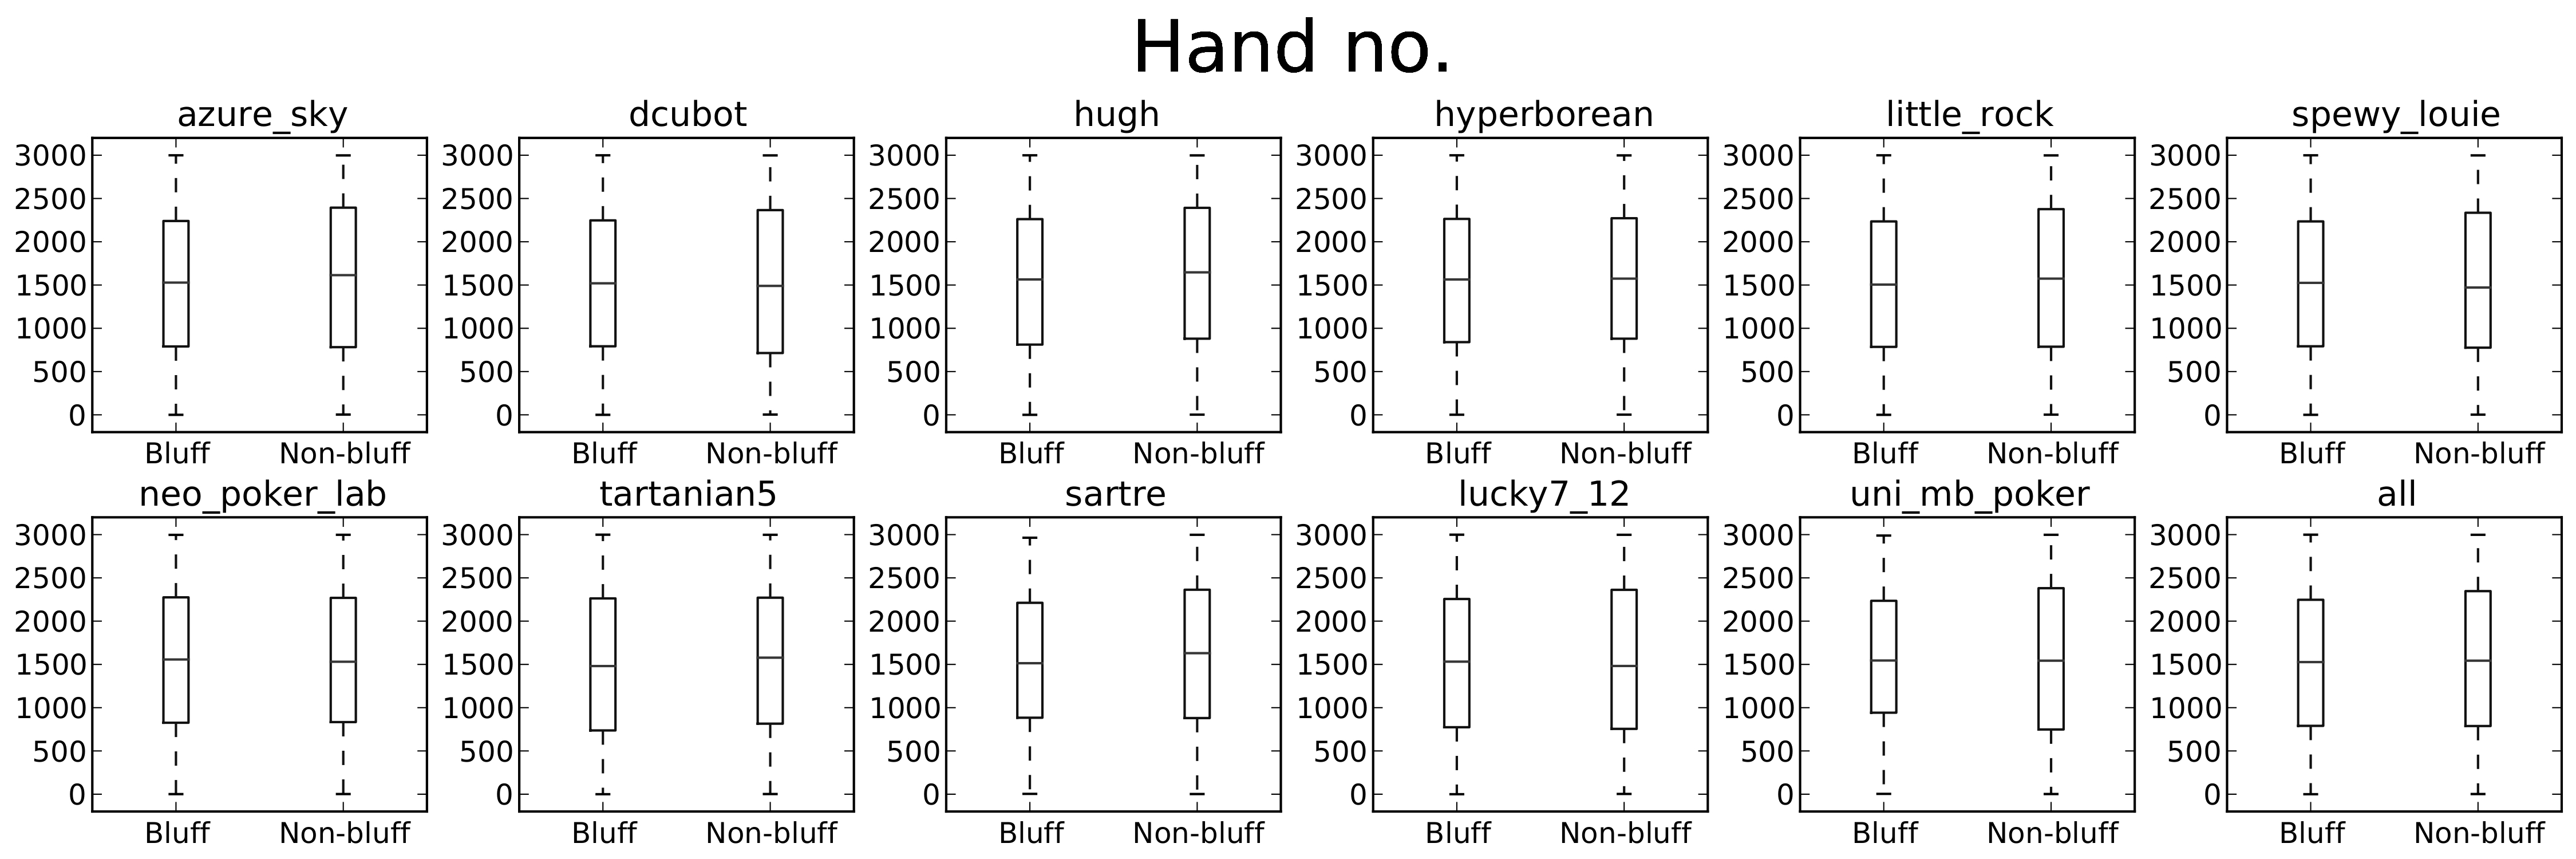
\includegraphics[width=\textwidth,natwidth=610,natheight=642]{handVarBW.jpg}
    \caption{The players don't appear to take much account of the game stage. We can see some slight differences in a few bots, such as tartanian5, who seems to make his bluffs slightly earlier in the game.}
\end{figure}

\begin{figure}[H]
    \centering
    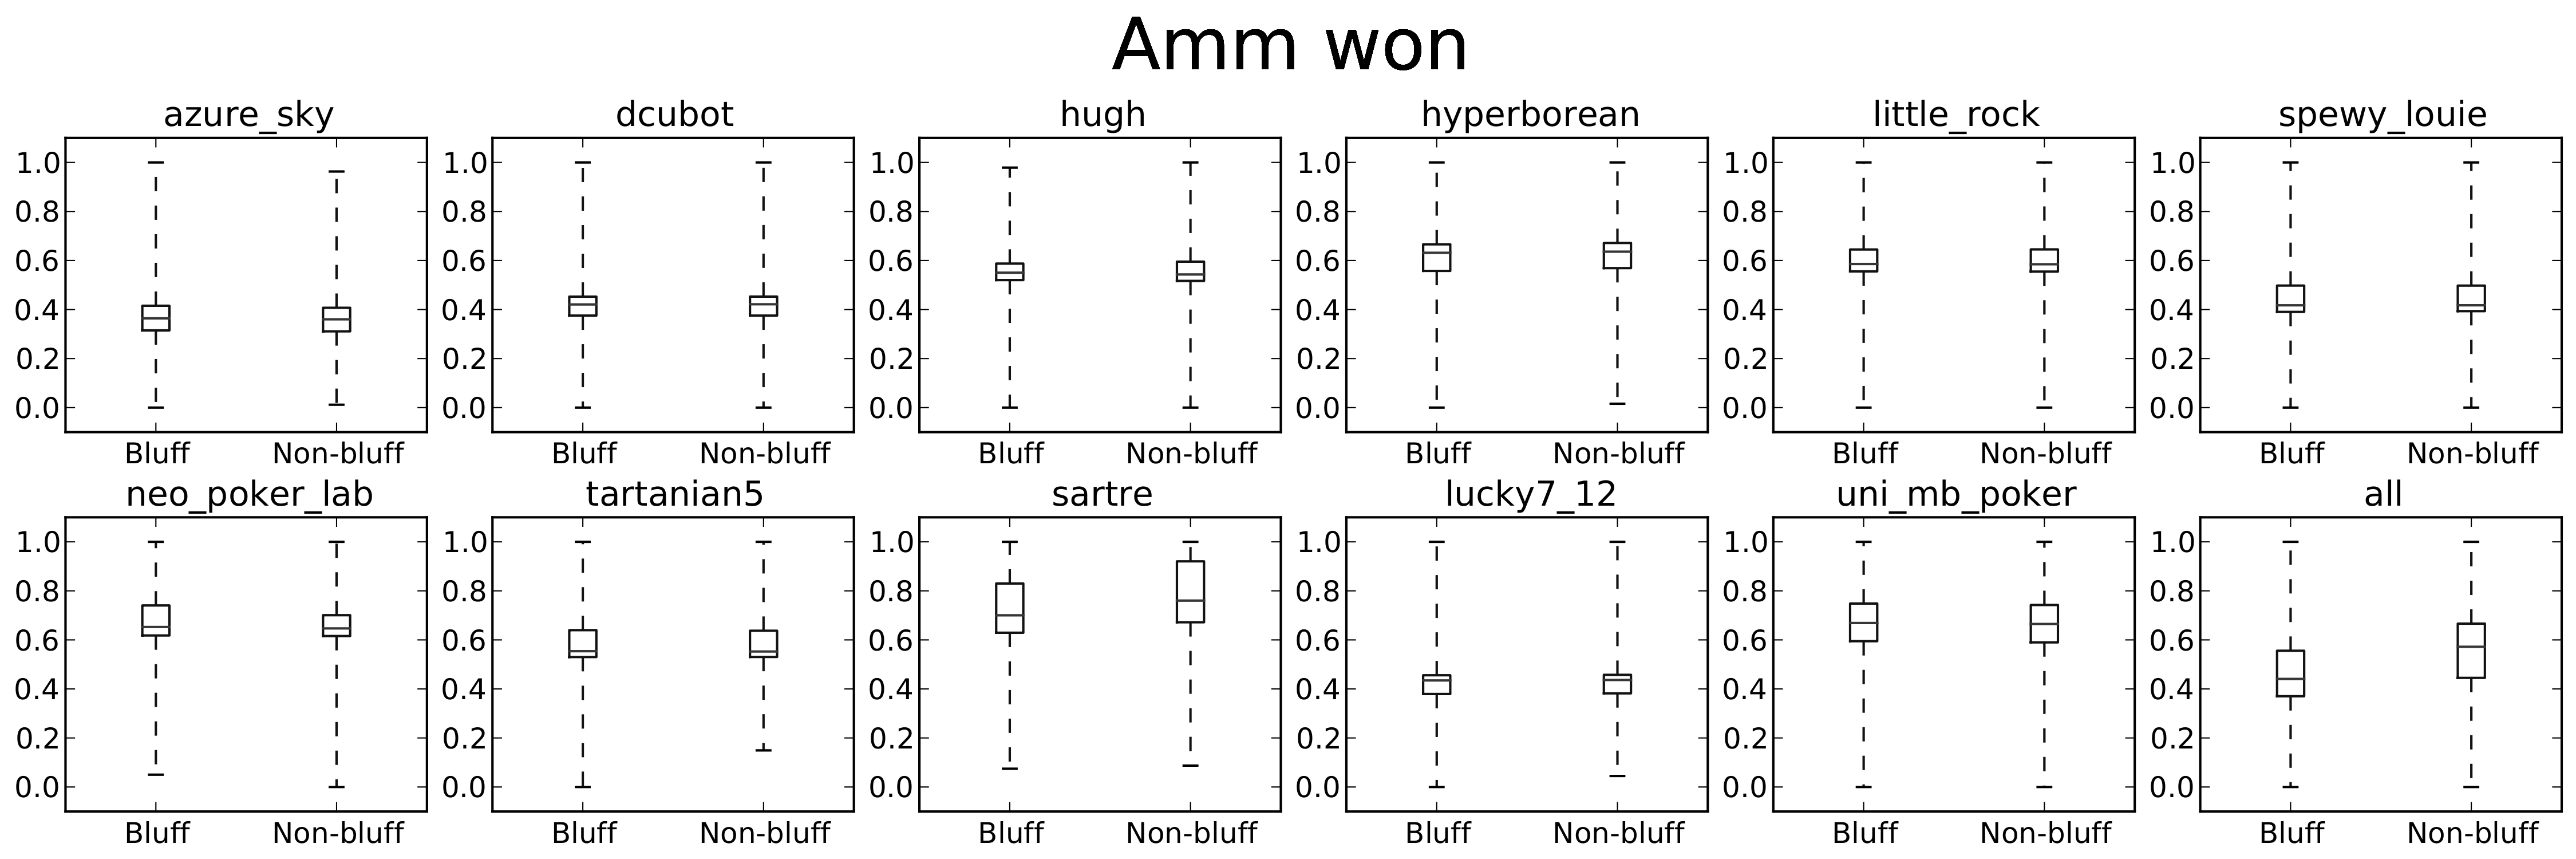
\includegraphics[width=\textwidth,natwidth=610,natheight=642]{histAmmWonBW.jpg}
    \caption{Here we see some interesting results. It looks like, almost universally, the bots are less likely to bluff if they've previously won similar hands. A possible explanation would be that when the bots are losing they are willing to take more risks and bluff more.}
\end{figure}

\begin{figure}[H]
    \centering
    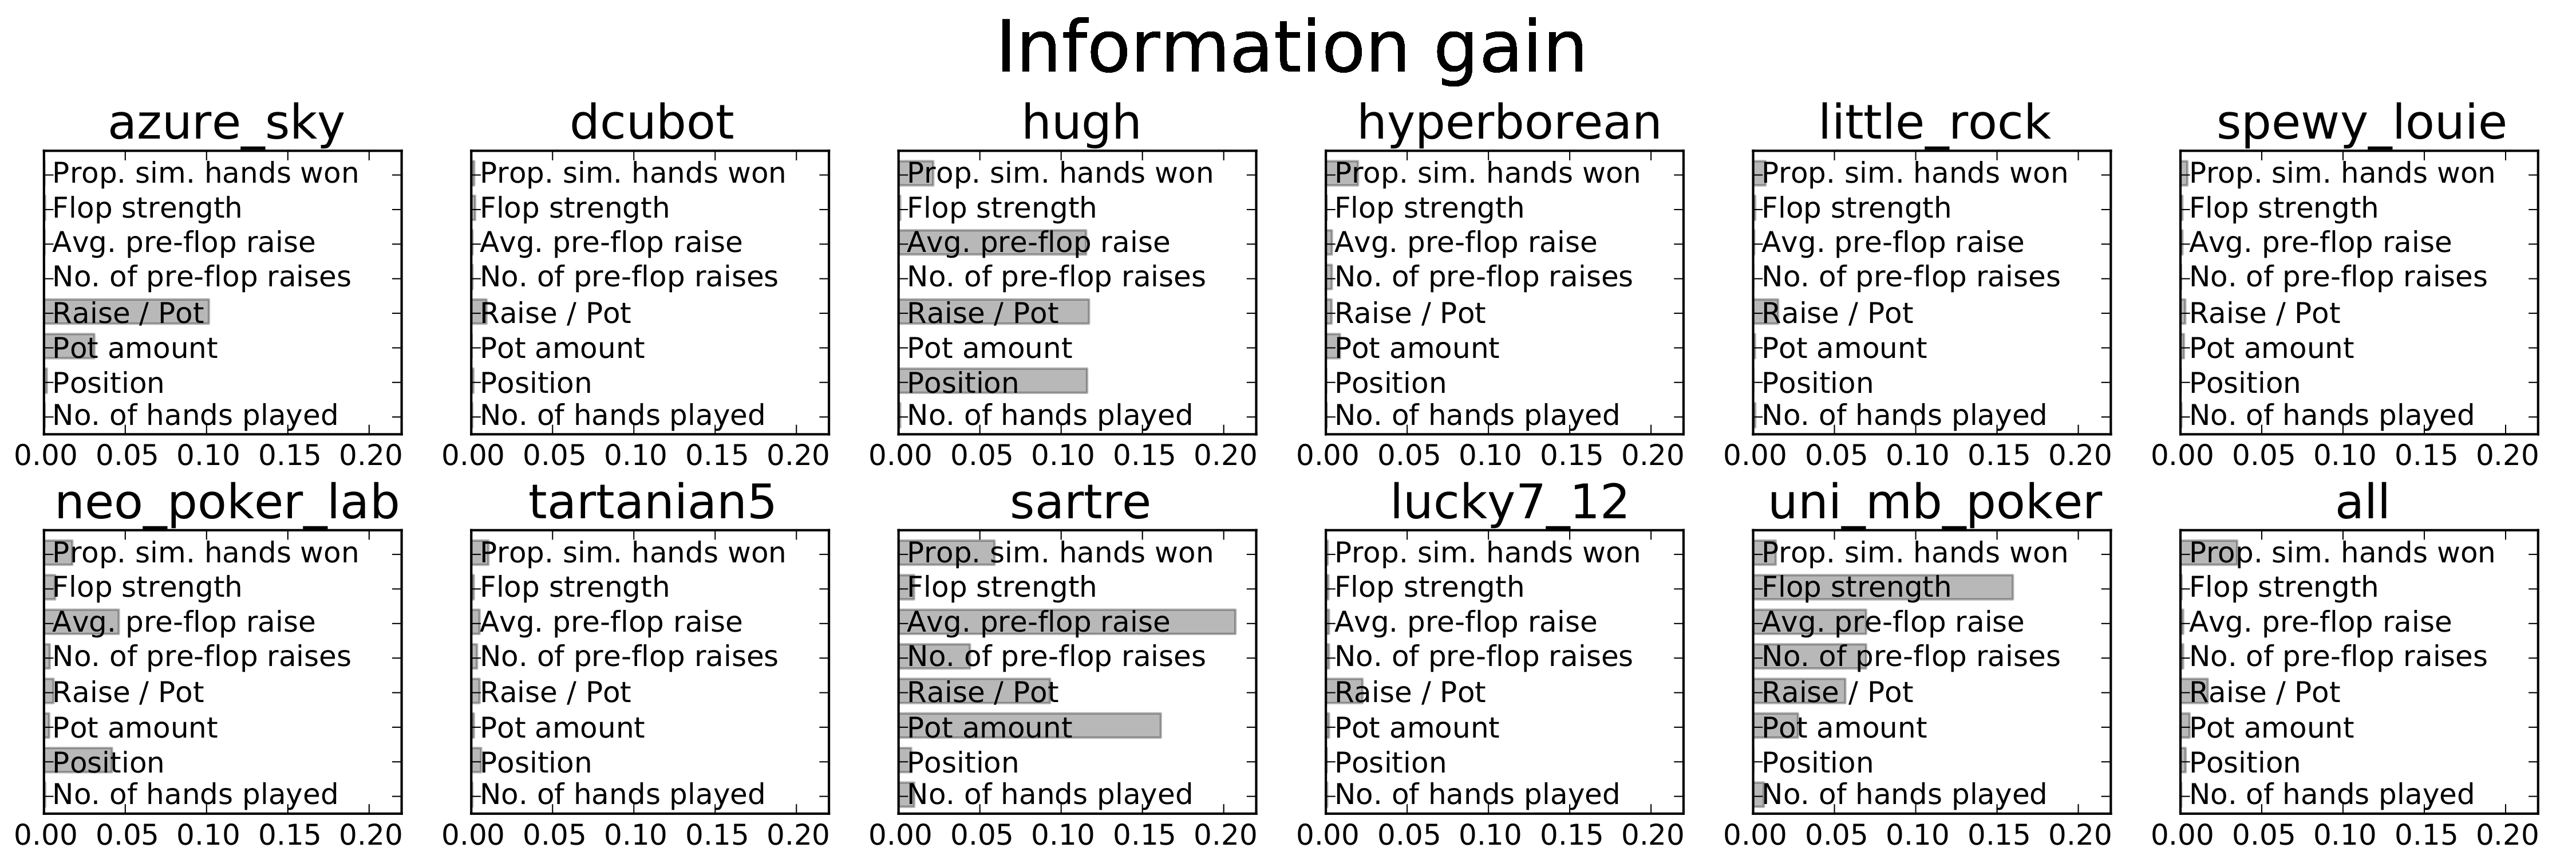
\includegraphics[width=\textwidth,natwidth=610,natheight=642]{ig8_200BW.jpg}
    \caption{The information gained by splitting the hands into two categories based on one feature.}
\end{figure}
\twocolumn
\section{
\fontsize{12pt}{15pt} 
\selectfont
Feature evaluation}
\fontsize{10pt}{12pt} 
\selectfont
The results shown in Figures 1 to 8 give us some insight into which features might be useful for which bots and why this is so. However, just looking at the distribution of the features does not allow us to quantify the comparative predictive power offered by any of them. One way to get a sense of the value they offer is to look at the classification problem from an information theoretic perspective. We can split the dataset into two categories, based on the values of the feature we are considering. We can then calculate the entropy of the initial distribution of bluff and non-bluff cases and the entropy of the two categories we have obtained by splitting the original dataset. By taking the weighted average of the entropies of said 2 categories, we can compare the initial entropy to the entropy obtained after splitting the hands and thus calculate the \emph{information gain}\footnote{Information gain is also known as the Kullback-Leibler divergence \cite{P14}} achieved by the split. 

Formally, if $X$ is a set of played hands and $x_f$ is a feature of one of the hands, then we can split the set $X$ into two categories as follows: 
\begin{gather*}
X_a(div) = \{x \in X | x_f <= div\} \\
X_b(div) = \{x \in X | x_f > div\}
\end{gather*}
If we further define $H(X)$ as the entropy of $X$ over bluffs and non-bluffs, then we can evaluate the information gain of this split by saying: 
\begin{align*}
IG(X,div) = & H(X) - \frac{|X_a(div)|}{|X|} H(X_a(div)) \\
 & - \frac{|X_b(div)|}{|X|} H(X_b(div))
\end{align*}
The problem with the above formulation is that most features are not binary and therefore it is unclear how to pick the $div$ value on which the split must be performed. We take a heuristic solution to this problem, which proves to be robust. We define the ``interesting range" of a feature's values as the range where the middle 80\% of values lie. We then do a uniform random sampling from this range, and keep the sample with the largest information gain. Experimental results show that increasing the number of samples from 100 to 2000 does not noticeably improve the information gain of any of the features on any of the bots, thus giving us some assurance as to the robustness of the method. The resulting observed information gains are shown in Figure 9. One of the interesting take-aways from this figure is that the features can have wildly different effectiveness levels on different bots. Another take-away, and obvious problem, is that on a few of the bots none of the features seem to have a significant impact. 

The issue here is that the information gain we have calculated is a lower bound on the predictiveness of the features. This is due to the fact that the features may have complex distributions which would require more than 1 division points to fully take advantage of. In order to get a better idea of the total effectiveness of all these features, we apply a decision tree algorithm to the task of classifying the hands into bluffs and non-bluffs. We first perform a further filtering step as to ensure that both bluffs and non-bluffs are equally represented in the results. This should allow the prediction results to be compared fairly across bots even if one of the agents tends to bluff more than another. We performed the classification task using 10-fold cross-validation, while ensuring that the folds are made as to preserve the proportions of the classes. The ROC curves are shown in Figure 10.

While the results presented in Figure 10 are quite good, a question arises regarding the speed of convergence to these results. If it takes us many thousands of hands of play to reach the above accuracies, then the features are not actually very useful when playing against a new opponent. In order to get a sense of the behavior of the classifier as the amount of data decreases, we analyze the change in the area under the ROC curve (which we call \emph{AUC}) as the amount of data changes. Since we're drastically reducing the size of our datasets, we want to make sure the variance of the results isn't too large. We therefore repeat the experiments on different subsets of the original dataset and average the results. As an example, for a test case containing 1\% of the data, we would run 100 simulations which would cover all of the original data, 1\% at a time. Additionally, each of these individual simulations also uses 10-fold cross-validation. Figure 11 shows the results obtained when the amount of data varies from 1\% to 100\% of the total. 

In order to highlight the performance obtained on very few training cases, Figure 12 shows the results when the size of the training set goes from 5 data points to 1000. As before, this data was generated by averaging repeated tests on subsets of the original datasets. Since some of these data subsets are very small, we use 3-fold cross-validation so that the training sets can have sufficient samples.

From both of these figures we can see that the convergence behavior of the AUC varies significantly from bot to bot. On agents such as azure\_sky and sartre, we can achieve highly reliable classification even with a very small number of training points. Conversely, on dcubot and spewy\_louie, even 1000 training cases only brings us up to an AUC of $\sim$0.6, whereas the full dataset takes us to over $\sim$0.8. This behavior may be determined by the features that prove most reliable for the respective agents, as the convergence rates for the individual features will likely vary.

\onecolumn
\begin{figure}[H]
    \centering
    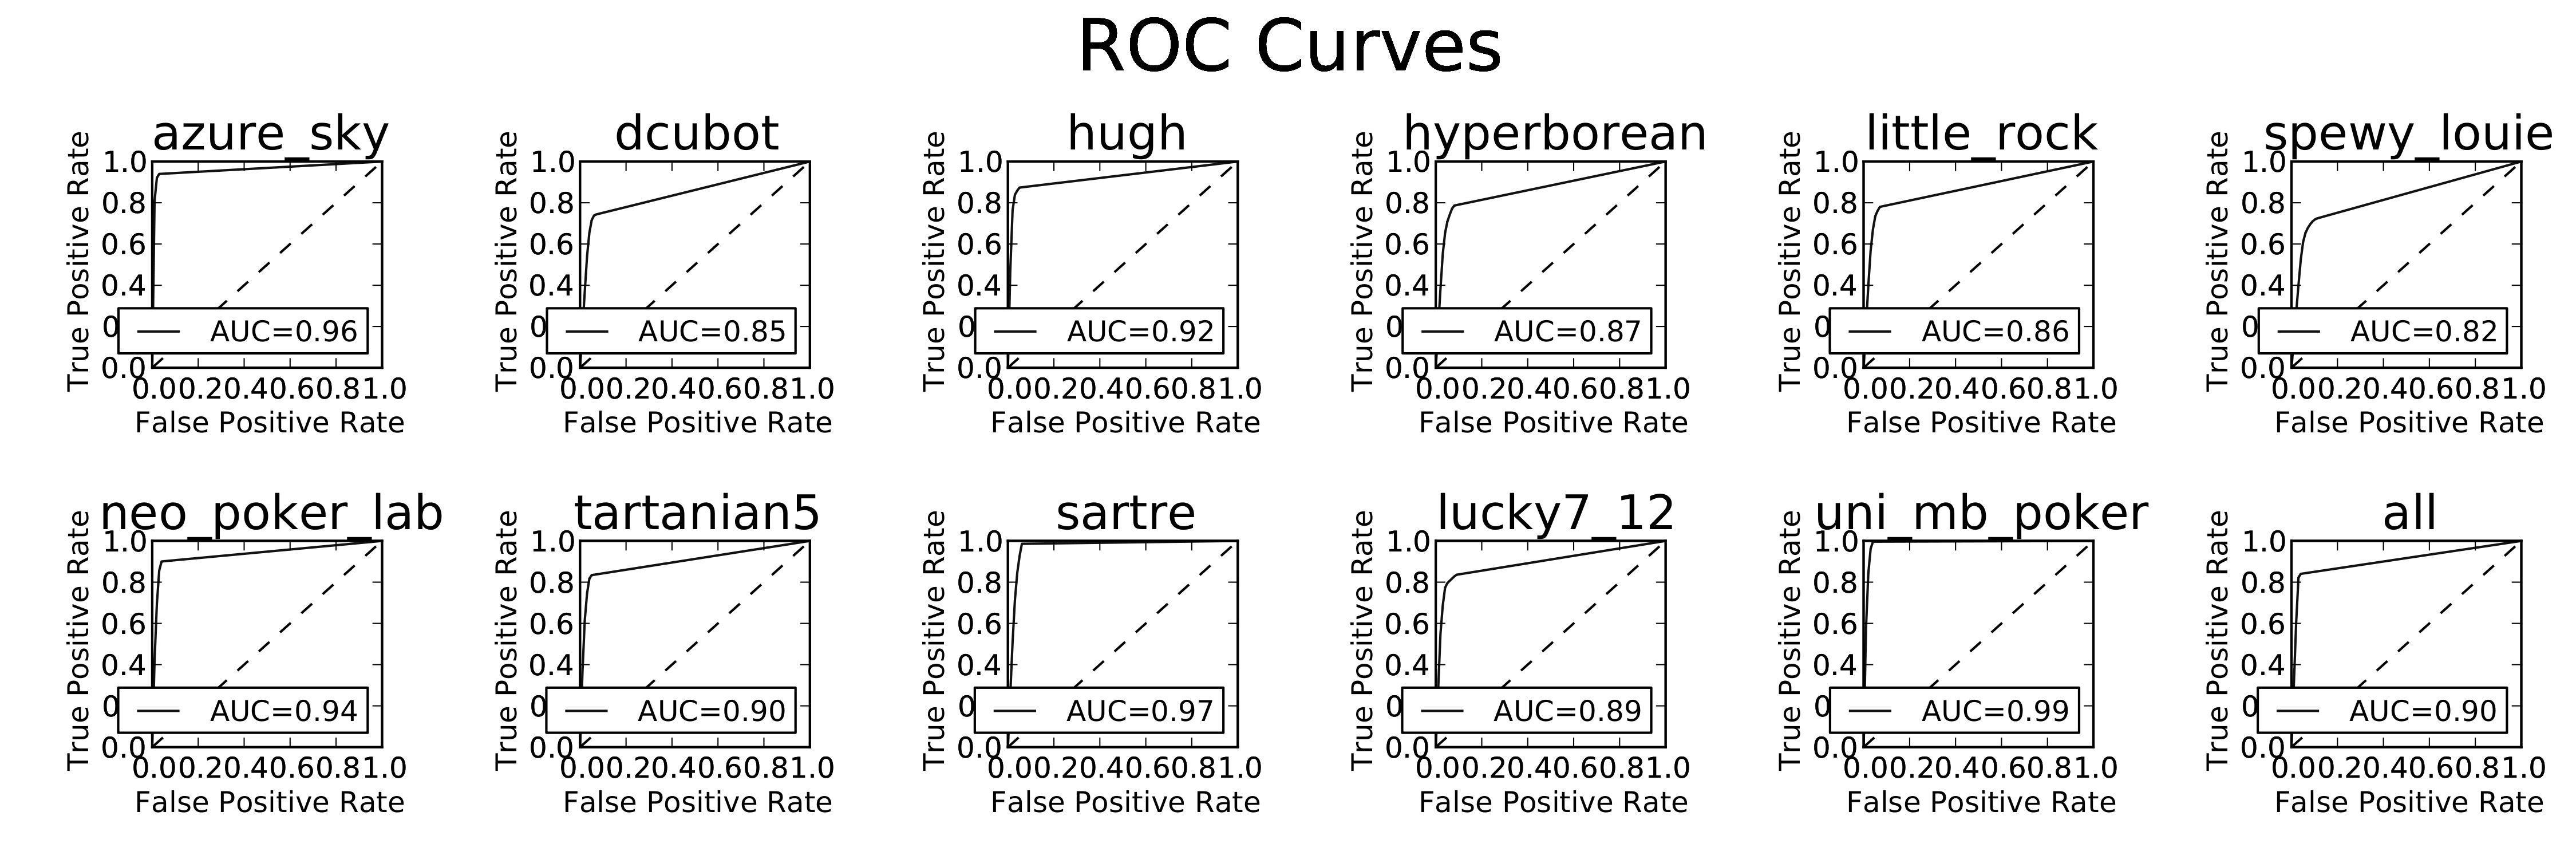
\includegraphics[width=\textwidth,natwidth=610,natheight=642]{rocNorm8BW.jpg}
    \caption{The ROC curves obtained by running a decision tree algorithm using the 8 aforementioned features.}
\end{figure}
\begin{figure}[H]
    \centering
    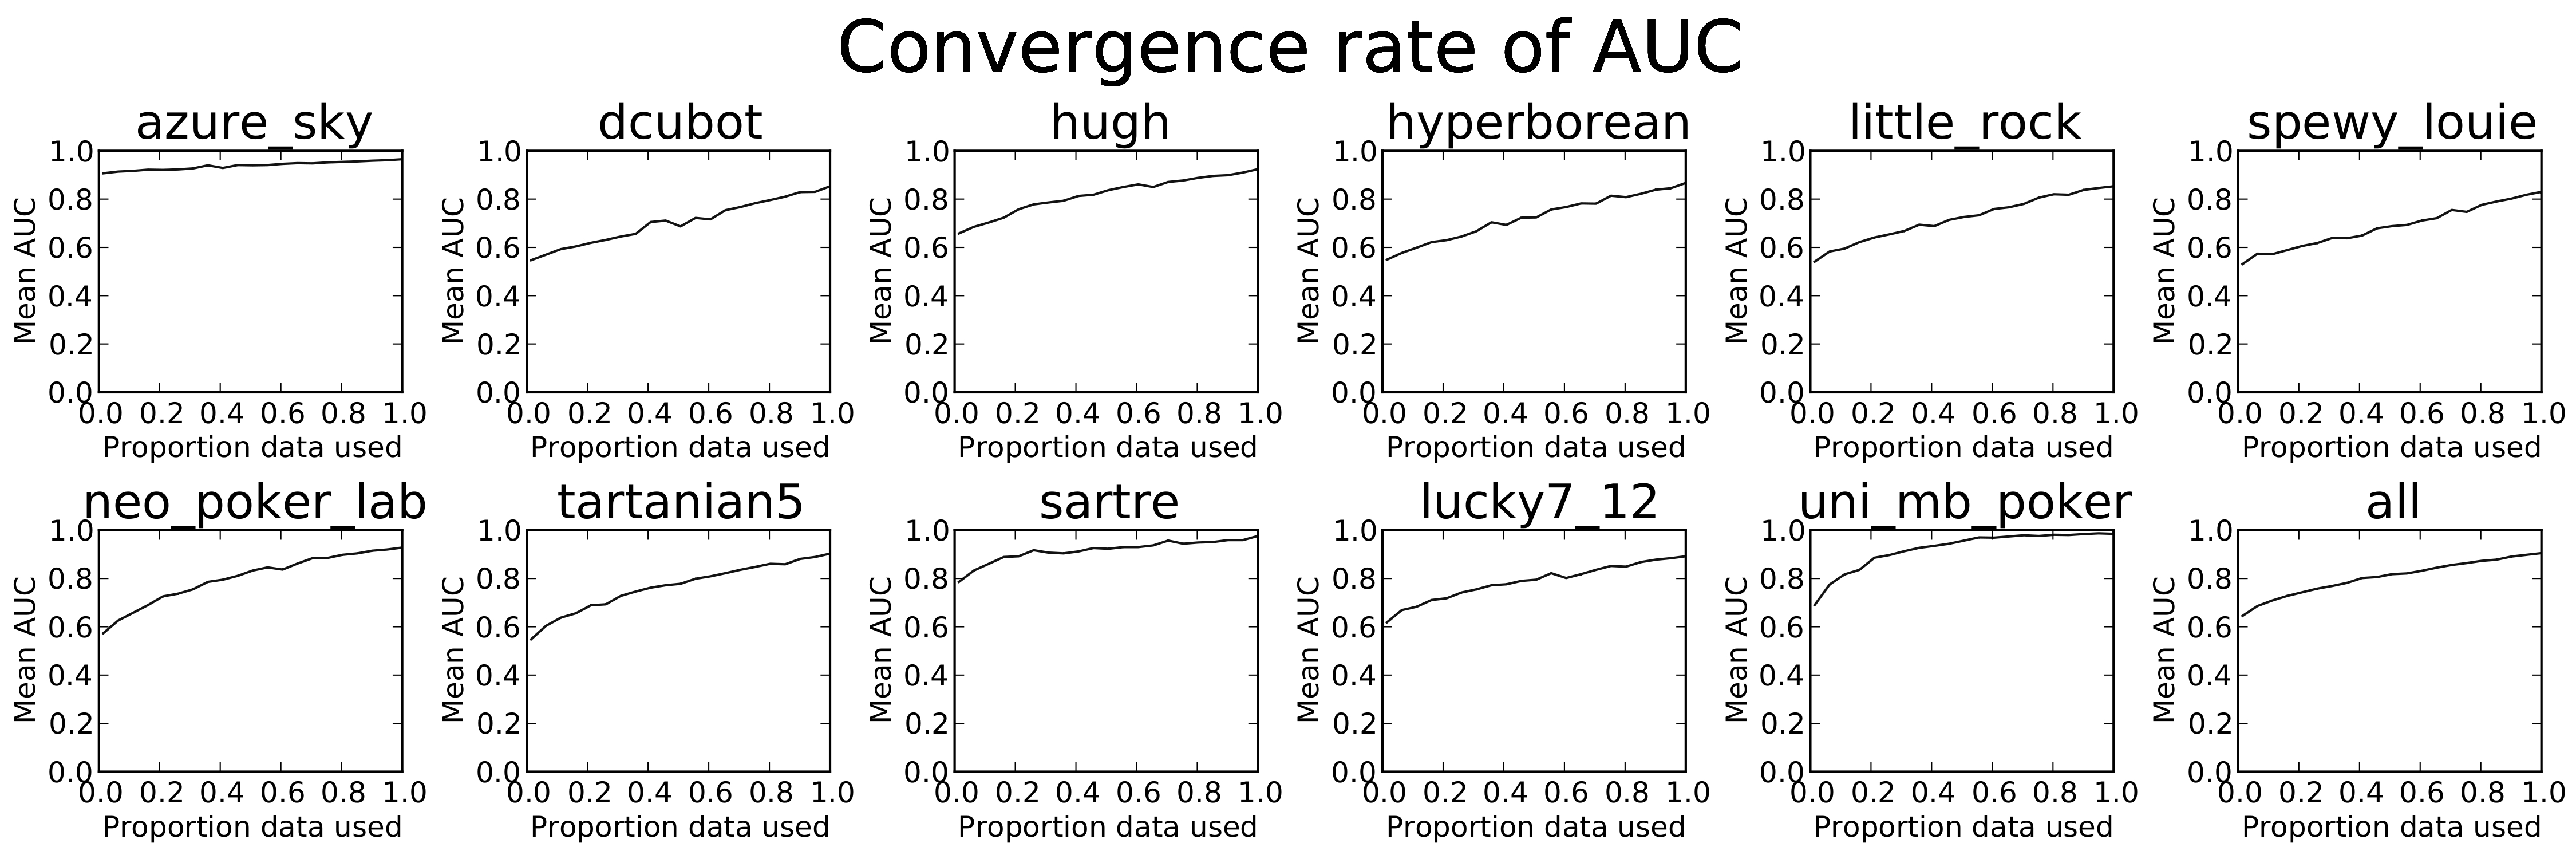
\includegraphics[width=\textwidth,natwidth=610,natheight=642]{convergence8BW.jpg}
    \caption{The convergence rate of the \emph{Area Under Curve} as the amount of data used grows from 1\% to 100\%.}
\end{figure}
\begin{figure}[H]
    \centering
    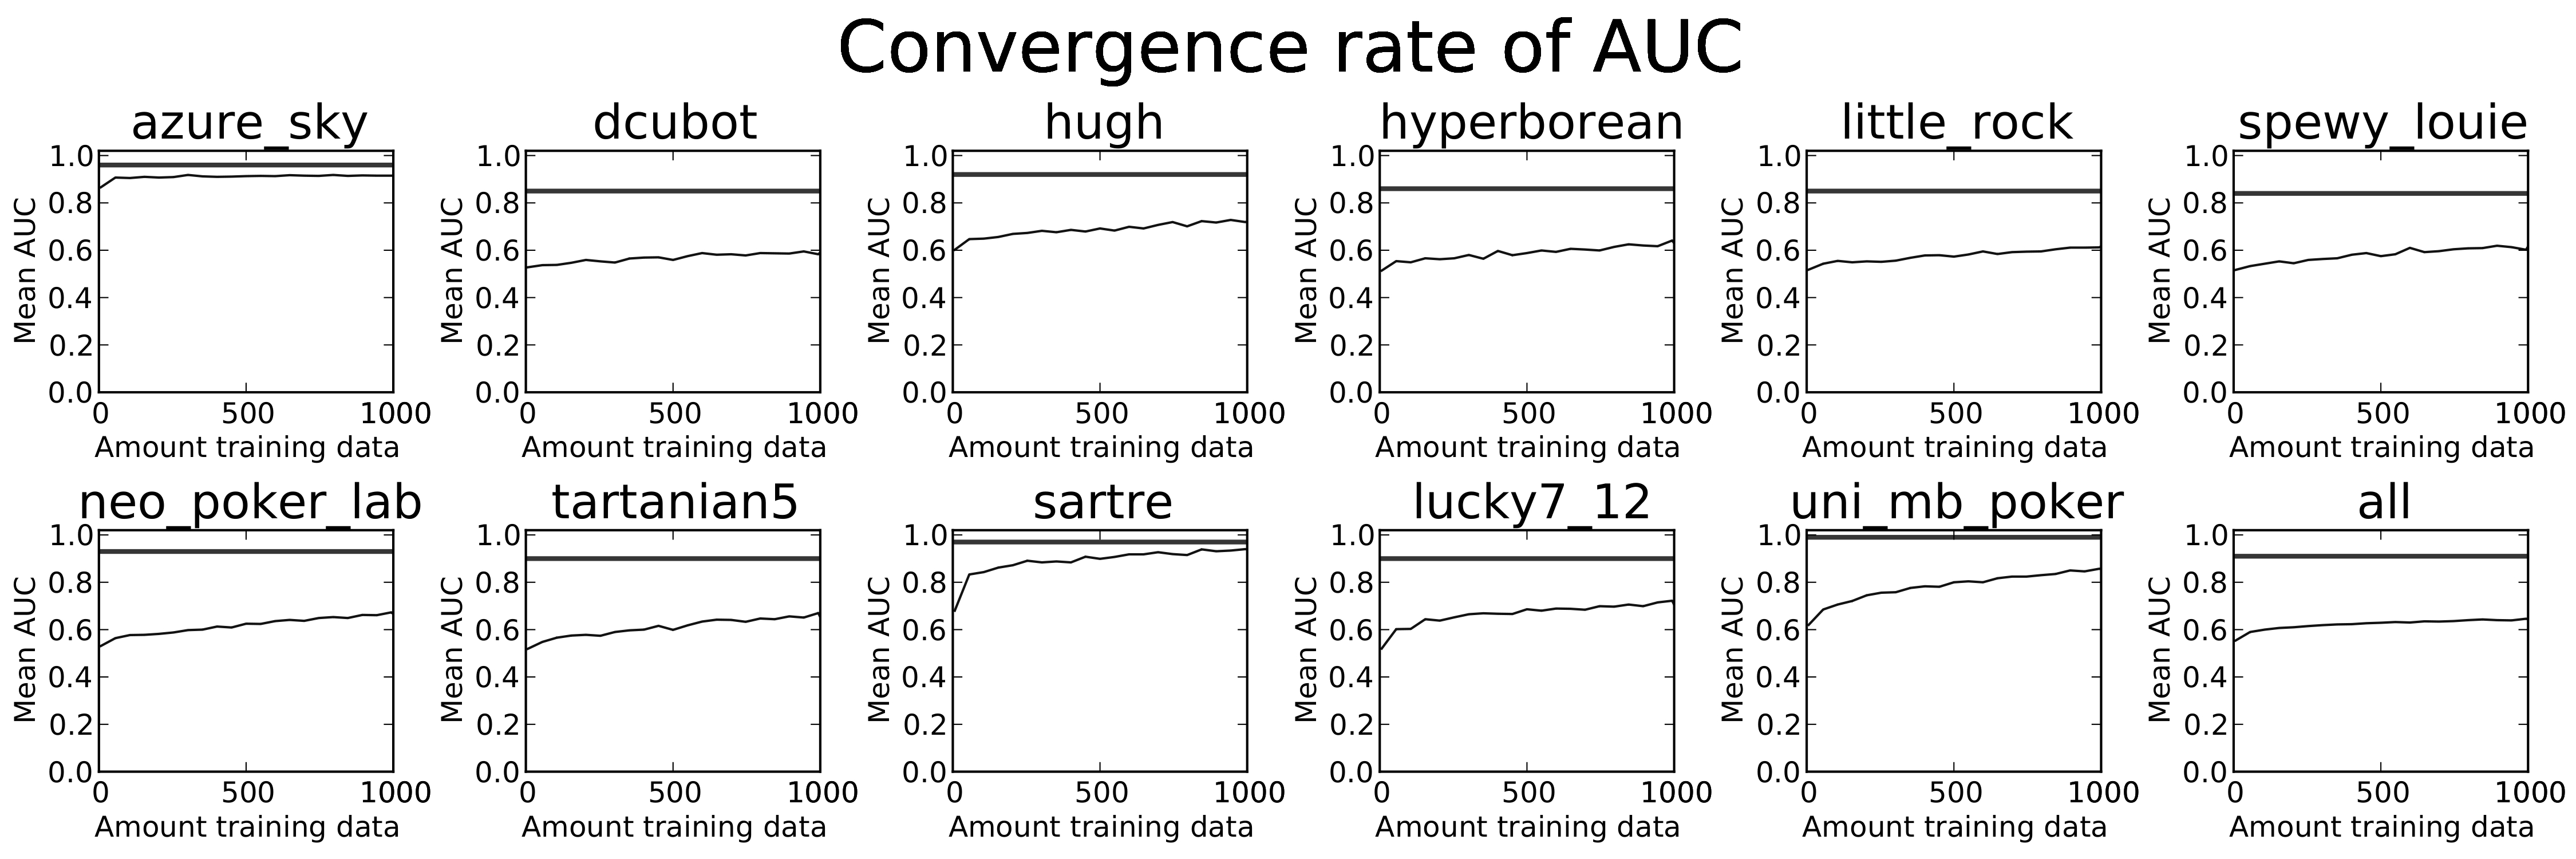
\includegraphics[width=\textwidth,natwidth=610,natheight=642]{smallConv8BW.jpg}
    \caption{A zoom in on the convergence rate on small amounts of training data, varying from 5 test cases to 1000. The horizontal line shows the AUC score obtained on the full dataset.}
\end{figure}
\twocolumn

\section{
\fontsize{12pt}{15pt} 
\selectfont
Conclusions and Future Work}
\fontsize{10pt}{12pt} 
\selectfont
We have formulated and analyzed several features for the purpose of bluff detection. This task was performed on the 11 agents that competed in the 2012 ACPC no-limit hold'em competition, as well as on an aggregate agent combining the previous 11. We looked at the way the distribution of features varies over the bluffs and non-bluffs, for each agent, and at how much information can be gained by classifying the dataset according to one of the features. Combining all the features in order to perform a classification gave us good results, even when using a basic, out-of-the-box, decision tree classifier. Finally, we have analyzed the robustness of this classifier as the amount of training data decreases, which has given us mixed results on the various agents.

From here. there are many potential avenues to explore. One obvious question is what causes the discrepancy between the analyzed agents, both regarding classification error and, especially, regarding robustness. The performance of the individual features should be evaluated as the amount of training data decreases and we should see if this might explain the different agent robustness levels. 

A limitation of the current approach is that we only use data directly related to our filtered hands in order to perform the classification. A natural extension is to try to infer information about the agent's bluffing habits from all played hands. This would require the design of further features which can capture aspects such as the opponent's general aggressivity and propensity for risk taking.

Other possible directions would include applying more complex machine learning techniques to the classification problem and extending the filtered hands to include more situations than the current flop flush scenario. Finally, the integration of these methods into the general opponent modelling framework should be considered.
%%%%%%%%%%
% References and End of Paper
\bibliographystyle{aaai}
\bibliography{poker}
\end{document}
